\subsection{Effetto del materiale sulla misura}

Abbiamo testato quanto la presenza di lastre di metallo potesse influire sulla rivelazione dei raggi cosmici,
per indagare quanto possa essere rilevante il materiale circostante (soffitto, pareti).
Abbiamo a disposizione:
\begin{itemize}
	\item 3 lastre di piombo rivestite di alluminio, ciascuna di spessore totale \SI{4}{mm},
	\item 1 lastra di alluminio di spessore \SI{4}{mm},
	\item 10 lastre di piombo spesse \SI{2}{mm}.
\end{itemize}
Non abbiamo misurato lo spessore della parte di piombo di quelle con piombo e alluminio.
Le lastre di metallo ricoprono circa l'\SI{80}\% delle lastre di scintillatore. 

\subsubsection{Conteggi}

Abbiamo posizionato le lastre di metallo tra il PM3 ed il PM4
per vedere se esse riuscivano a fermare parte dei muoni.
Per fare questa misura abbiamo confrontato il rapporto tra le coincidenze 5\&4\&3 e 5\&4
al variare del numero di lastre di metallo.
Abbiamo confrontato i rapporti per non dover tener conto dell'accettanza%
\footnote{Sia l'efficienza che la geometria.}.

\begin{table}[h]
\centering
\begin{tabular}{| c | r @{$\pm$} l | r @{$\pm$} l | r @{$\pm$} l |}
\hline
tempo totale [\si{s}] & \multicolumn{2}{c|}{R($C2$) [1/\si{s}]} & \multicolumn{2}{c|}{R($C2\cdot \delta$) [1/\si{s}]} & \multicolumn{2}{c|}{R($C3$) [1/\si{s}]} \\
\hline
1030 & 19.6&0.1 & 12.92&0.09 & 13.1&0.1 \\
1030 & 19.8&0.1 & 13.00&0.09 & 12.9&0.1 \\
1030 & 19.8&0.1 & 13.00&0.09 & 13.1&0.1 \\
1000 & 20.1&0.1 & 13.19&0.09 & 12.7&0.1 \\
\hline
\end{tabular}
\caption{MODIFICARE:
colonna 1: lastre usate;
colonna 2: conteggio c2;
colonna 3: conteggio c3;
colonna 4: c3/c2 con l'errore giusto}
\label{dati cfr}
\end{table}


\begin{figure}[h]
\centering
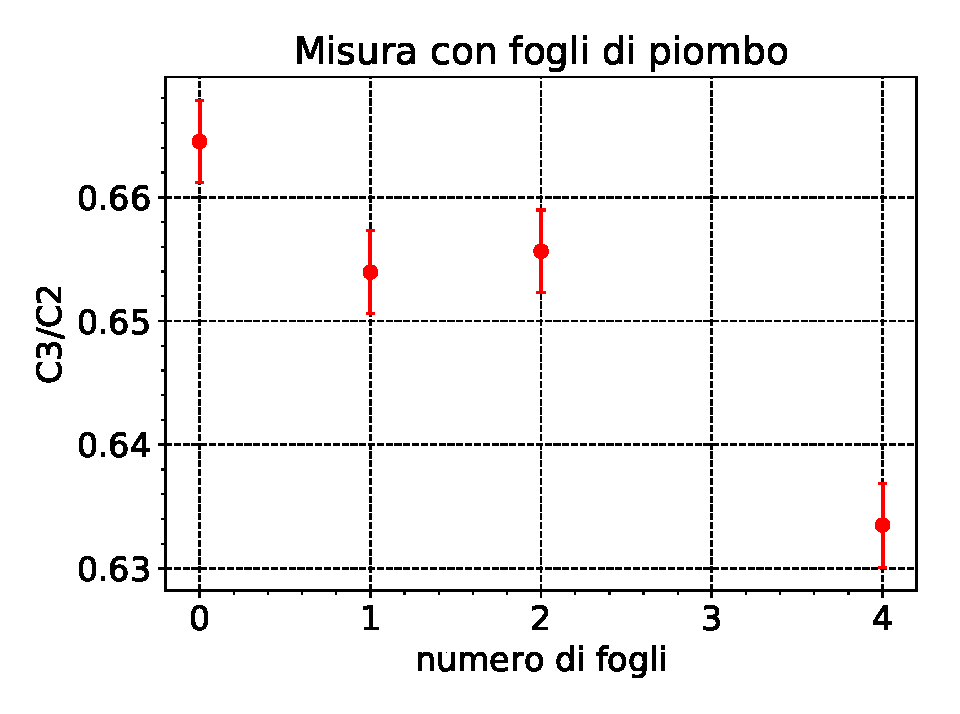
\includegraphics[width=8 cm]{confronto}
\caption{Rapporto tra coincidenze a 3 ($C3$) e coincidenze a 2 ($C2$) in funzione delle lastre di materiale inserite.}
\label{cfr}
\end{figure}

\subsubsection{Energia}

\begin{figure}
	\hspace{-7.5em}
	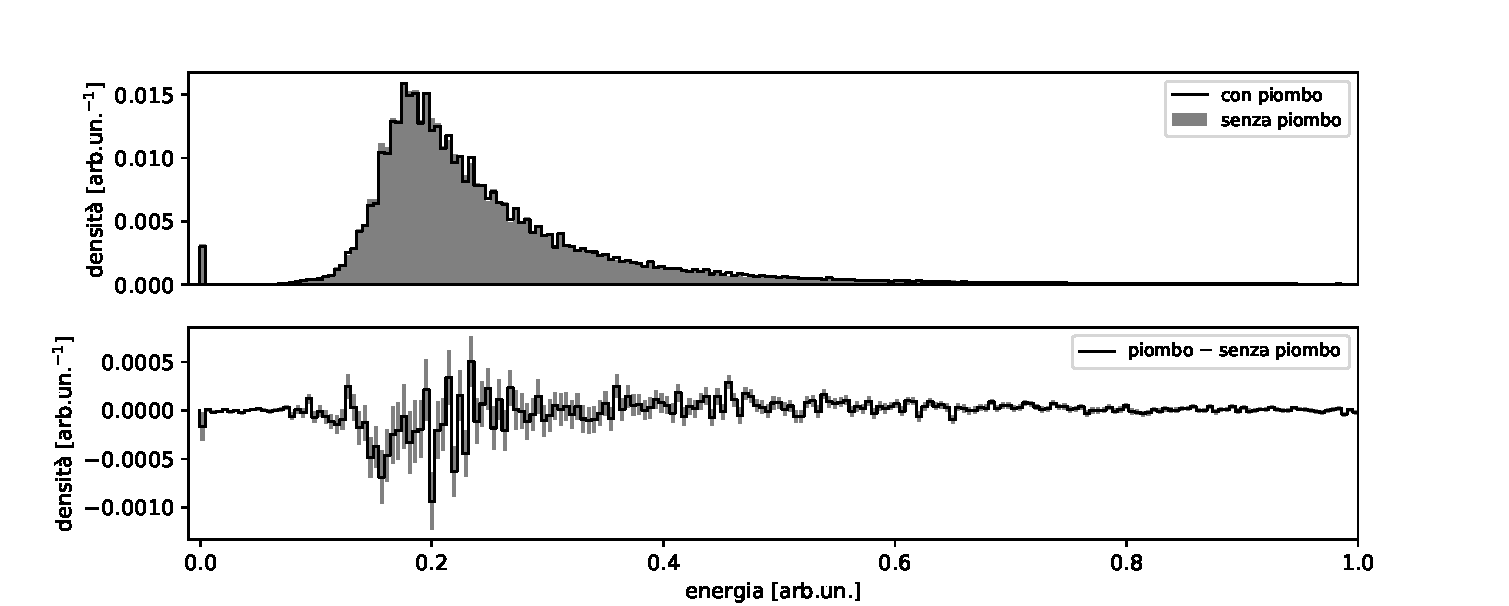
\includegraphics[width=1.4\textwidth]{piombo_energia}
	\caption{\label{fig:piomboenergia}
	Distribuzione del rilascio di energia sul PM1 con e senza lastre di piombo.
	L'istogramma ha un numero di bin pari alla radice quadrata del numero di campioni nella presa dati con meno campioni.
	Nel secondo grafico (la differenza degli istogrammi del primo)
	le barre d'errore sono riportate ma sono effettivamente molto piccole.}
\end{figure}

Infine abbiamo eseguito due acquisizioni di lunga durata.
Nella prima abbiamo messo tutte le lastre a nostra disposizione sul PM1
e abbiamo acquisito i loro rilasci di energia per tutta la notte.
Il giorno seguente le abbiamo tolte ed abbiamo preso dati per \SI{4}{ore}.
In entrambi i casi il trigger dell'ADC è dato dalle coincidenze PM2 \& PM1.

Il risultato è riportato in \autoref{fig:piomboenergia}.
Dal grafico della differenza delle distribuzioni
si nota che la distribuzione con il piombo è spostata verso energia maggiore.
È in effetti plausibile che i muoni rallentati dal piombo
rilascino più energia a causa della risalita di ionizzazione.
Per verifica confrontiamo i due campioni con il test di Kolmogorov-Smirnov a $5\sigma$,
risulta significativo.
\marginpar{Dovremmo parlare del fatto che la distribuzione è irregolare (i picchetti non sono statistici).
Controllare che non siano per la discretizzazione dell'ADC (allineare i bin ai digit).}
